Det må man sige at han er, og derfor er der ikke nogle grund til at lave
rastte af resultaterne da han bare kan ændre på virkeligheden.

Vi har køre vores naive algoritme på 20 snit i det horisontale og
vertikale plan og kommer frem til 2 grafer over summeringen af alle
regioner fundet i vært snit. 

Man kan se i grafen \ref{antal_regioner_vertikale_cut} for det vertikale
plan, at regionerne koncentrationen sig omkring miden af billederne.

I grafen for den horisontale plan \ref{antal_regioner_horisontale_cut}
er der 3 snit som udskiller sig fra resten $91\%$, $61\%$ og $56\%$.
Hvor $91\%$ ligger højest. Fra miden af billedet og op af bliver der
fundet færre og færre regioner i snittene. Det kan skyldes at billeder med hoisont normalt ikke har mange regioner over hoisonden, men mange under hoisonden, eller at vores algoritme regner forkert, det første er nok det meste sansyndlige, da vores algoritme iterere hoisontal i gemme maleriet nå vi skal finde hoisontal regioner og vertikal nå vi finder vertikal regioner, så er eventuel type fejl i algoritmen vil også kunne ses i den anden graf \ref{antal_regioner_vertikale_cut}.

Hvis man samler informatioerne for de 2 grafer, kan man se at regionerne
samler sig fra den horisontale miden og ned af i billedet med peaker i
miden af det vertikalle plan. Det mod skrider hypotese \ref{hypoet_alle_andre_snit},\ref{hypo_midten} 
og vi kan derfor forkaste dem.

I graferne kan vi også se at det gyldne snit $G$ har samme antal eller
flere regioner en $\frac{2}{3}$, som approksimmeret i grafen er $36$ og
$66$, derfor er hypotese \ref{hypo_to_tredjedele} sand og kan derfor ikke forkastes.

\begin{figure}[h!]
	\begin{center}
		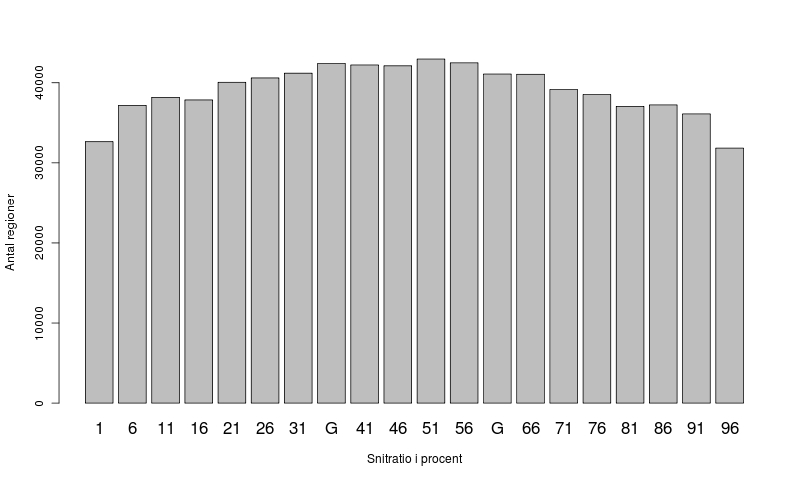
\includegraphics[width=0.9\textwidth]{afsnit/resultater/billeder/cut0cut1eatsperratio.png}
	\end{center}
	\caption{Antal regioner i hvert af de 20 vertikale snit}
	\label{antal_regioner_vertikale_cut}
\end{figure}

\begin{figure}[h!]
	\begin{center}
		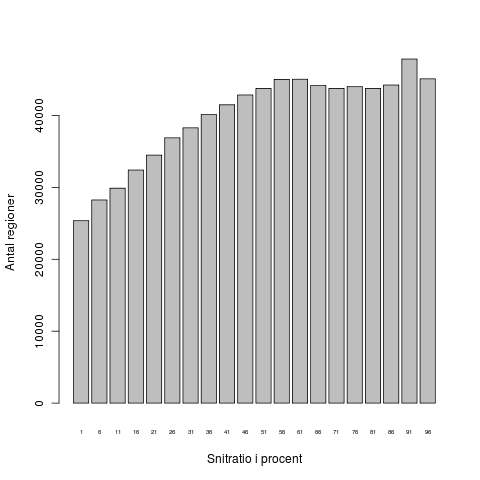
\includegraphics[width=0.9\textwidth]{afsnit/resultater/billeder/cut2cut3eatsperratio.png}
	\end{center}
	\caption{Antal regioner i hvert af de 20 horisontale snit, hvor venstre side af grafen repræsentere øverst del af malerierne}
	\label{antal_regioner_horisontale_cut}
\end{figure}
